% LaTeX2e Template by Stephen Iota (https://stepheniota.com/)
% last updated: Jan. 2019

% for papers
%\documentclass[aps,onecolumn,superscriptaddress]{revtex4-1}
% https://www-d0.fnal.gov/Run2Physics/WWW/templates/revtex4.pdf
% https://cdn.journals.aps.org/files/revtex/auguide4-1.pdf
% for revTeX4-1 class options

% for other
\documentclass[10pt]{article}
\usepackage[margin=3cm]{geometry}

%%%%%%%%%%%%%%%%
%%% Packages %%%
%%%%%%%%%%%%%%%%

\usepackage[utf8]{inputenc}
\usepackage{amsmath}
\usepackage{amssymb}
\usepackage{amsfonts} % to remove math font when typesetting equations
\usepackage[thinc]{esdiff} 
\usepackage{graphicx}
\usepackage[shortlabels]{enumitem} % to change labels in enum/item
\usepackage[dvipsnames]{xcolor} % for colored links

% always put this at the end
\usepackage[
	colorlinks=true,
	citecolor=green!50!black,
	linkcolor=NavyBlue!75!black,
	urlcolor=green!50!black,
	hypertexnames=false]{hyperref} 

 
 %%%%%%%%%%%%%%%%%%
 %% New Commands %%
 %%%%%%%%%%%%%%%%%%
 
\newcommand{\email}[1]{\texttt{\href{mailto:#1}{#1}}}

\newcommand{\hint}[1]{\color{Blue}{#1}}
 
%----------------------------------------------------
%%%%%%%%%%%%%%%%%%
%% Front Matter %%
%%%%%%%%%%%%%%%%%%

\pagenumbering{gobble} % no page numbers
\graphicspath{{figures/}} % set directory for figures
%\usepackage{wrapfig}
%\setcounter{section}{-1} % start with section 0

%%%%%%%%%%%%%
%%% Title %%%
%%%%%%%%%%%%%
\begin{document}

\begin{center}

\Large{\textsc{Week 1}: \textbf{Motion in Physics}}

\end{center}

\vspace{.5mm}


%%%%%%%%%%
%% INFO %%
%%%%%%%%%%

\begin{tabular}{rl}
\textsc{SI Leader}:
&
Stephen Iota (\email{siota001@ucr.edu})
\\
\textsc{Course}:
&
Physics 40A (Winter 2019), Prof.~John Ellison
\\
\textsc{Date}:
&
9 January 2019
\end{tabular}

%%%%%%%%%%%%%%
%% PROBLEMS %%
%%%%%%%%%%%%%%

\section{Kinematic Equations}

Write down the five kinematic equations. Identify which two are the fundamental equations. 


\section{Motion Diagrams}

Three motion diagrams are shown. Draw an acceleration vs time and a velocity vs time graph for each.
\begin{center}
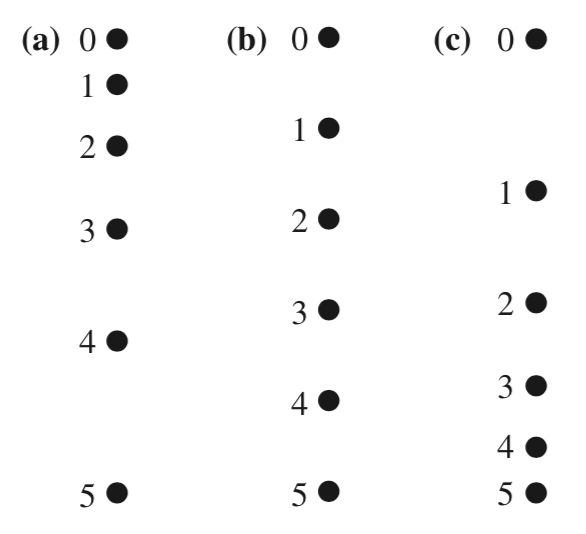
\includegraphics[width=.3\linewidth]{PS1-FigA}
\end{center}

\section{Velocity Diagram}

Indicate on the graph where objects 1 and 2 have the same velocity.
\begin{center}
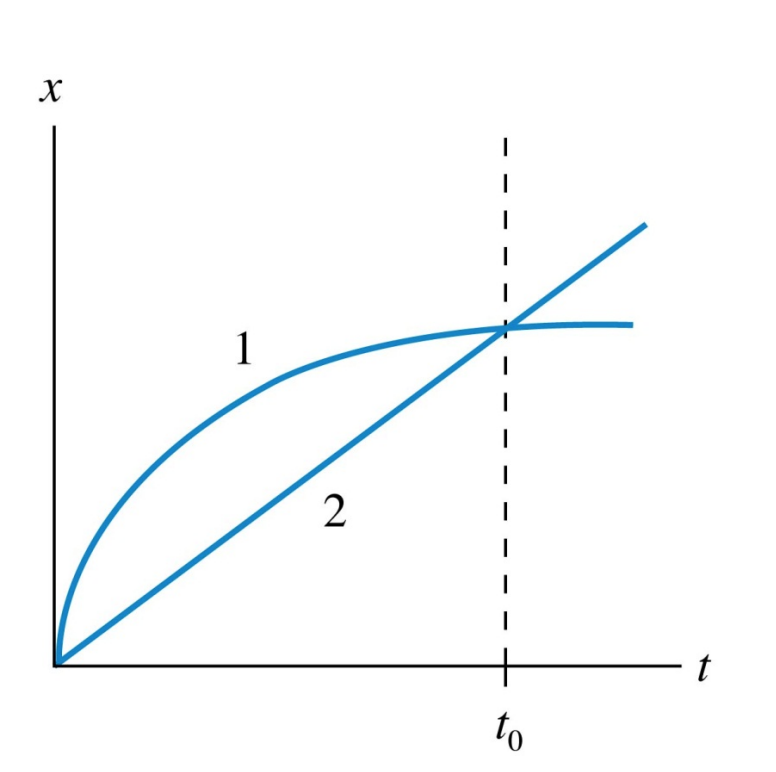
\includegraphics[width=.3\linewidth]{PS1-FigB}
\end{center}

\section{Stopping at a Red Light}

A motorist is traveling at 20 m/s. He is 60 m from a stoplight when he sees it turn yellow. His reaction time, before stepping on the brake, is 0.50 sec. What steady deceleration while braking will bring him to a stop at the red light? 

\section{Logarithmic Acceleration}

A car accelerates logarithmically ($\vec{a}(t) = \ln{t} \ \hat{x}$). Solve for position as a function of time $x(t)$.

\end{document}